% !TEX program = xelatex

\documentclass{noithesis}

\begin{document}

\title{浅谈支配树及其应用}
\author{南京外国语学校\ 陈孙立}

\maketitle

\begin{abstract}
	
	本文主要介绍了支配树的求解算法以及它的应用。
	
	本文第二节介绍了一些记号和定义。
	
	本文第三节着重讲解了支配树的求解算法。
	
	本文第四节介绍了支配树的一些应用。
	
	本文第五节是总结。
	
\end{abstract}

\section{引言}

支配树这个概念在图论和计算机设计理论中经常出现,作为一个算法也时有出现在各类算法竞赛中,但是系统介绍它的中文资料却相对较少。笔者希望通过本文,能让更多的同学了解支配树,以及它的一些应用。

\section{定义}

本文中我们考察一个 $n$ 个点 $m$ 条边的\textbf{有向图} $G = (V, E)$ ,其中 $V$ 是节点集,$E$ 是边集,且 $|V| = n, |E| = m$ 。本文假设读者已经熟悉图论中路径、环、深度优先搜索(DFS)、拓扑序、DFS序等基础概念。

在给定一个源 $s\in V$ 的前提下,如果对于两点 $x,y$ 满足任意以 $s$ 为起点,$y$ 为终点的路径都经过 $x$ ,则称 $x$ 支配(dominates) $y$ 。由于当不存在 $s$ 到 $x$ 的路径时,和 $x$ 有关的支配关系都没有意义,所以\textbf{在本文中,我们始终假设从 $s$ 能到达所有其他点},对于一般的图只需先以 $s$ 为起点进行深度优先遍历,并只保留被访问的点即可。

首先观察到,我们可以仅考虑简单路径,这是因为如果路径出现了重复节点,可以把重复部分之间的节点删去,这样的修改对支配条件不会产生影响。一个显然的性质是 $s$ 支配所有点,除此之外,支配关系还满足以下性质,从而可以用一个树结构完全描述它们。

\textbf{性质1}:如果 $x$ 支配 $y$ 且 $y$ 支配 $z$ 则 $x$ 支配 $z$ ,也即支配关系满足\textbf{传递性}。

这个性质比较显然。

\textbf{性质2}:如果 $x$ 支配 $y$ 且 $y$ 支配 $x$ ,则 $x=y$ 。

\textbf{证明}:假设 $x\neq y$ ,可知任意一条从 $s$ 到 $x$ 的简单路径都经过 $y$ ,且在经过 $y$ 之前必须经过 $x$ ,于是这条路径形如 $s,\dots,x,\dots,y,\dots,x$ ,和简单路径矛盾。由此导出必有 $x=y$ 。\qed

\textbf{性质3}:如果 $x,y,z$ 互不相等,且 $x$ 和 $y$ 均支配 $z$ ,则必有 $x$ 支配 $y$ 或 $y$ 支配 $x$ 。

\textbf{证明}:考察任意一条从 $s$ 到 $z$ 的简单路径,这条路径上必有 $x$ 和 $y$ ,不失一般性可以假设路径形如 $s,\dots,x,\dots,y,\dots,z$ 。如果 $x$ 不支配 $y$ ,则存在一条不经过 $x$ 的 $s$ 到 $y$ 的路径,此时若把前述路径从 $s$ 到 $y$ 的部分替换成这条不经过 $x$ 的路径,就得到了一条从 $s$ 到 $z$ 且不经过 $x$ 的路径了,而这和 $x$ 支配 $z$ 矛盾。\qed

上述性质表明,对于某点 $x\neq s$ ,考察点集 $S = \{y\mid y\text{ 支配\ }x\}$ ,则 $S$ 中的点依支配关系构成全序集,且 $S$ 中有至少两个元素。由此,一定存在一个点 $z$ 满足:如果 $y\neq x$ 支配 $x$ ,则 $y$ 也支配 $z$ 。我们称 $z$ 是 $x$ 的直接支配点(immediate dominator),记为 $z=idom(x)$ 。

现对于所有除 $s$ 之外的点 $x$ 连一条 $idom(x)\rightarrow x$ 的边,这样得到的图每个点的入度均不超过 $1$ ;结合\textbf{性质1}和\textbf{性质2}可知,这个图是无环的,于是这样的图一定是一个以 $s$ 为根的有向树,称为支配树(Dominator Tree),记为 $DT(G, s)$ 。它满足:对于两点 $x,y$ ,$x$ 支配 $y$ 当且仅当在支配树上 $x$ 是 $y$ 的祖先(本文中的祖先等于自身),所以只要得到了支配树,我们就得到了所有的支配关系。

\begin{figure}[h]
	\centering
	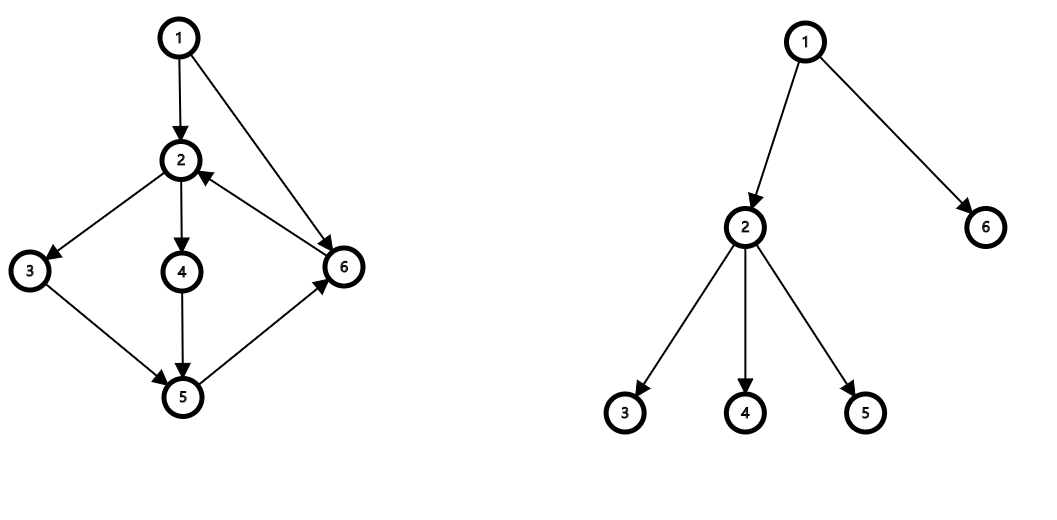
\includegraphics[width=0.9\textwidth]{graph2.png}
\end{figure}

下面右图是左图在 $s=1$ 时的支配树。

\section{支配树的求解算法}

\subsection{有向无环图的特殊情况}

对于有向无环图 $G = (V, E)$ ,由于拓扑序在后的点不会影响前面点的支配关系,可以按照拓扑序依次求解每个点 $x$ 的直接支配点。现假设所有拓扑序在 $x$ 之前的点的直接支配点都已求出,此时可以得到一个不完整的支配树,它一定是最终得到的支配树的一部分,这里姑且叫做“当前支配树”。设以 $x$ 为终点的边有 $(c_1,x),\dots,(c_k,x)$ ,则 $idom(c_i)$ 均已求出。

\textbf{引理1}:点 $y$ 支配 $x$ 当且仅当 $y=x$ 或 $y$ 支配所有 $c_1,\dots,c_k$ 。

\textbf{证明}:$y=x$ 时结论显然,下面假设 $y\neq x$ 。先证当 $y$ 支配所有 $c_1,\dots,c_k$ 时,$y$ 必支配 $x$ :考察任意一条从 $s$ 到 $x$ 的路径,则在 $x$ 之前的点一定是 $c_1,\dots,c_k$ 之一,于是这条路径必须经过点 $y$ 。

再证上面的否命题:不失一般性假设 $y$ 不支配 $c_1$ ,则存在从 $s$ 到 $c_1$ 的路径不经过 $y$ ,此时可以沿这条路径走到 $x$ ,就得到了一条从 $s$ 到 $x$ 的、不经过 $y$ 的路径,于是 $y$ 不支配 $x$ 。\qed

满足上面性质的点就是 $c_1,\dots,c_k$ 在“当前支配树”上的公共祖先,于是 $idom(x)=LCA(idom(c_1), \dots, idom(c_k))$ (LCA指最近公共祖先),这相当于在“当前支配树”上添加了一个叶子和一条边。如果使用倍增求解LCA的算法,只需稍加修改就能支持每次添加一个叶子了,这个做法的时间和空间复杂度都是 $O((n+m)\log n)$ 。

\subsection{半支配点的定义和性质}

在之后的算法中我们要考虑任意一个图 $G$ 的从 $s$ 出发的DFS树,即进行深度优先遍历时经过的边形成的树结构,同时按照遍历顺序(DFS序)为点赋予大小。具体来说对于两点 $x,y$ ,如果 $x$ 在遍历时比 $y$ 访问的时间更早,则称 $x<y$ ,类似地也可定义 $x>y$ ,以及点集的最大值和最小值等相关概念。有向图的DFS树不存在边 $(x, y)$ 满足 $x<y$ 且 $x$ 不是 $y$ 的祖先。一个更有用的表述是:

\textbf{定理1}:如果 $x\le y$ 则任意 $x$ 到 $y$ 的路径必须经过 $x$ 和 $y$ 在DFS树上的某个公共祖先。

\textbf{证明}:$x$ 是 $y$ 的祖先时结论显然,因此可认为 $x$ 不是 $y$ 的祖先。假设存在一条路径 $x=v_0, v_1,\dots, v_k=y$ ,其中不存在 $x$ 和 $y$ 在DFS树上的公共祖先。令 $z$ 是 $x$ 和 $y$ 在DFS树上的最近公共祖先, $z$ 的孩子中必有唯一一点 $y'$ 是 $y$ 的祖先。

考察任意一条路径 $x=v_0, v_1, \dots, v_k = y$ ,令 $p=\max\{i\mid v_i<y'\}$ ,并假设 $v_p$ 不是 $z$ 的祖先,那么 $v_p$ 也一定不是 $v_{p+1}$ 的祖先,这是由DFS序的性质得到的:若 $x$ 是 $y$ 的祖先,则 $x$ 也是 $z(x\le z\le y)$ 的祖先。由此可得存在边 $(v_p, v_{p+1})$ 且 $v_p<v_{p+1}$ ,$v_p$ 不是 $v_{p+1}$ 的祖先。然而,这条边不可能在DFS树中存在,否则在遍历到 $v_p$ 时会直接沿着这条边遍历 $v_{p+1}$ 。这个矛盾表明 $v_p$ 一定是 $z$ 的祖先。\qed

下面给出半支配点(semi-dominator)的定义。

\textbf{定义}:点 $x$ 的半支配点 $sdom(x) = \min\{y \mid\text{ 存在一条路径\ }y=v_0,v_1,\dots,v_k=x\text{ 满足对于任意\ }1\le i\le k-1\text{ 都有\ }v_i>x\}$ 。

称定义中路径的存在性为“半支配点条件”。半支配点的求解是直接支配点求解的中间步骤。以下是一些关于直接支配点和半支配点的重要性质。

\textbf{引理2}:$idom(x)$ 和 $sdom(x)$ 都是DFS树上 $x$ 的祖先且不等于 $x$。更进一步地,在DFS树上 $idom(x)$ 是 $sdom(x)$ 的祖先。

\textbf{证明}:$idom(x)$ 在DFS树上是 $x$ 的祖先是显然的,因为DFS树上有一条 $s$ 到 $x$ 的路径,$idom(x)$ 必定在这条路径上。

由于 $x$ 在DFS树上的父亲已经满足了半支配点的要求,所以有 $sdom(x)<x$ 。另一方面,如果 $sdom(x)$ 不是 $x$ 的祖先,则不难发现 $sdom(x)$ 在DFS树上的父亲也满足半支配点的要求,且比 $sdom(x)$ 更小,这和半支配点的定义矛盾。

根据半支配点的定义,可以沿DFS树从 $s$ 走到 $sdom(x)$ 再沿定义所述的路径走到 $x$ 。因此DFS树中,$sdom(x)$ 到 $x$ 的路径上(这里不包括 $sdom(x)$)的点均不支配 $x$ ,故 $idom(x)$ 一定是 $sdom(x)$ 的祖先。\qed

\textbf{引理3}:令 $v,w$ 满足DFS树上 $v$ 是 $w$ 的祖先,则 $v$ 是 $idom(w)$ 的祖先或 $idom(w)$ 是 $idom(v)$ 的祖先。

\textbf{证明}:若 $v=w$ 结论显然,因此假设 $v\neq w$ 。使用反证法,由于$v, w, idom(v), idom(w)$ 都是 $w$ 的祖先,如果引理中的结论不成立,则它们按深度排序依次是 $idom(v), idom(w), v, w$ 且它们互不相等。这意味着存在一条不经过 $idom(w)$ 的从 $s$ 到 $v$ 的路径,继续沿DFS树走到 $w$ 就得到一条不经过 $idom(w)$ 的从 $s$ 到 $w$ 的路径,矛盾。\qed

有了上述性质,我们将展示半支配点和直接支配点的紧密联系,从而可以通过前者计算后者。

\textbf{定理2}:任取点 $w\neq s$ 。考虑DFS树上从 $sdom(w)$ 到 $w$ 的路径上(不包括 $sdom(w)$)的任意点 $x$,如果均满足 $sdom(x)\ge sdom(w)$ ,则 $idom(w)=sdom(w)$ 。

\textbf{证明}:根据\textbf{引理2},有 $idom(w)$ 是 $sdom(w)$ 的祖先,因此只需证 $sdom(w)$ 支配 $w$ 。考虑任意一条 $s$ 到 $w$ 的路径 $P$ ,我们将要证明 $sdom(w)$ 一定在 $P$ 中。令 $x$ 是 $P$ 中\textbf{最后一个}满足 $x < sdom(w)$ 的点,如果不存在则必有 $sdom(w) = idom(w) = s$ ,结论仍然成立。同时,令 $y$ 是 $P$ 中 $x$ 之后的第一个在DFS树中从 $sdom(w)$ 到 $w$ 的路径上的点。在 $P$ 中截取 $x$ 到 $y$ 之间的部分得 $v_0 = x, v_1,\dots, v_k = y$。

现在考虑路径 $v_0,\dots,v_k$ ,我们声称对于 $1\le i<k$ 都有 $v_i > y$ ,也即 $sdom(y) \le x<sdom(x)$ 。若不满足这一点,则有某个 $v_i<y$ ,此时根据\textbf{定理1}可得存在某个 $i\le j\le k-1$ 满足 $v_j$ 是 $y$ 的祖先。由 $x$ 的取值可知 $sdom(w) \le v_j$ ,于是 $v_j$ 也在DFS树中从 $sdom(w)$ 到 $w$ 的路径上,这和 $y$ 的取值矛盾。上述矛盾可推得 $sdom(y)\le x < sdom(x)$ ,结合定理的条件必有 $y = sdom(w)$ ,即路径 $P$ 包含 $sdom(w)$。\qed

\textbf{定理3}:任取点 $w\neq s$ 。考虑DFS树上从 $sdom(w)$ 到 $w$ 的路径上(不包括 $sdom(w)$)的所有点,令 $u$ 是其中 $sdom$ 最小的点,则 $sdom(u)\le sdom(w)$ 且 $idom(u) = idom(w)$ 。

\textbf{证明}:由于 $w$ 也是 $u$ 的一个候选, $sdom(u)\le sdom(w)$ 是显然的。注意到在DFS树上 $idom(w)$ 是 $u$ 的祖先,于是根据\textbf{引理3}可知 $idom(w)$ 也是 $idom(u)$ 的祖先,因此只需证 $idom(u)$ 支配 $w$ 。考虑任意一条 $s$ 到 $w$ 的路径 $P$ ,我们将要证明 $idom(u)$ 一定在 $P$ 中。令 $x$ 是 $P$ 中\textbf{最后一个}满足 $x < idom(u)$ 的点,如果不存在则必有 $idom(u) = idom(w) = s$ ,结论仍然成立。同时,令 $y$ 是 $P$ 中 $x$ 之后的第一个在DFS树中从 $idom(u)$ 到 $w$ 的路径上的点。在 $P$ 中截取 $x$ 到 $y$ 之间的部分得 $v_0 = x, v_1,\dots, v_k = y$。

和\textbf{定理2}的证明类似,我们可以得到 $sdom(y)\le x$ 。根据\textbf{引理2}有 $idom(u)\le sdom(u)$ ,综合起来可得 $sdom(y)\le x<idom(u)\le sdom(u)$ 。至此,由 $u$ 的选择可知 $y$ 不能是 $sdom(w)$ 的除自身外的后代;另一方面,$y$ 不能既是 $idom(u)$ 的除自身外后代也是 $u$ 的祖先,否则沿DFS树从 $s$ 走到 $sdom(y)$ 再沿 $P$ 走到 $y$,最后沿DFS树走到 $u$ 的这条路径就不经过 $idom(u)$ 了,这和支配点的定义矛盾。

根据 $idom(u)\le sdom(w) < u\le w$ 和 $idom(u) < y$ ,唯一的情况就只剩下 $y = idom(u)$ 了,于是路径 $P$ 包含 $idom(u)$ 。\qed

上面两个定理说明了半支配点和直接支配点的关系,也给出了由前者求出后者的方法。对于点 $w\neq s$ 来说,考虑DFS树上从 $sdom(w)$ 到 $w$ 的路径上(不包括 $sdom(w)$)的所有点,令 $u$ 是其中 $sdom$ 最小的点,若 $sdom(u) = sdom(w)$ 则可利用\textbf{定理2}得到 $idom(w) = sdom(w)$ ;否则 $u\neq w$ ,可利用\textbf{定理3}得到 $idom(w) = idom(u)$ 。

\subsection{计算半支配点和直接支配点}

\subsubsection{半支配点}

为了求出半支配点,我们需要下面的定理。

\textbf{定理4}:$sdom(w)$ 由以下两种情况产生的候选取最小值得到。

\begin{itemize}
	\item 1. 有边 $(v,w)$ ,此时 $v$ 是 $sdom(w)$ 的候选。
	\item 2. $u$ 是 $v$ 在DFS树上的祖先,$u > w$ 且有边 $(v,w)$ ,此时 $sdom(u)$ 是 $sdom(w)$ 的候选。
\end{itemize}

\textbf{证明}:令 $x$ 是所有候选的最小值。我们首先证明每个候选都满足半支配点的条件,从而得到 $sdom(w)\le x$ 。若 $x$ 由情况1得到,则显然 $(x,w)$ 就是满足半支配点条件的路径;否则 $x = sdom(u)$ ,此时取出 $sdom(u)$ 到 $u$ 的半支配点条件中所述的路径,再接上DFS树中 $u$ 到 $v$ 的路径,最后从 $v$ 到 $w$ 就是满足 $w$ 的半支配点条件的路径。

还需证明 $sdom(w)\ge x$ 。为此考虑 $sdom(w)$ 到 $w$ 的半支配点条件对应的路径 $v_0=sdom(w), v_1, \dots, v_k = w$ ,其中对于任意 $v_i(1\le i<k)$ 都有 $v_i\ge w$。若 $k=1$ 则它在情况1中被考虑到,下设 $k > 1$ 。取 $j$ 是最小的满足 $j\le 1$ 且 $v_j$ 是 $v_{k-1}$ 在DFS树上的祖先的数,这样的 $j$ 一定存在,因为 $k$ 就是一个合法的数。

现在考虑路径 $v_0,\dots,v_j$ ,我们声称它是满足 $v_j$ 的半支配点条件的路径,即对于任意 $1\le i<j$ 都有 $v_i > v_j$ 。若不是,则考虑所有 $v_i\le v_j$ 的 $i$ ,取其中满足 $v_i$ 最小的 $i$ ,可由\textbf{定理1}得到 $v_i$ 一定是 $v_j$ 的祖先,这和 $j$ 的选取矛盾。于是 $sdom(v_j)\le sdom(w)$ ,而 $sdom(v_j)$ 必定在情况2中被考虑到,因此 $x\le sdom(w)$ 。\qed

有了\textbf{定理4},可以设计如下求出半支配点的算法:

\begin{itemize}
	\item 1) 求出图 $G$ 的一个DFS树和DFS序。
	\item 2) 若当前所有点的 $sdom$ 都已经求出,则结束算法;否则找到 $sdom(w)$ 未求出的点中最大的 $w$ 。
	\item 3) 考虑情况1,可以直接计算所有的候选。
	\item 4) 考虑情况2,枚举边 $(v,w)$ 且 $v > w$ ,此时 $v$ 一定被标记。从 $v$ 开始不断地在DFS树上向被标记的父亲走形成一条路径,并求出这条路径上 $sdom$ 的最小值作为候选。
	\item 5) 合并情况1和情况2求出的所有候选,得到 $sdom(w)$ 的值,标记 $w$ 为已求出 $sdom$ ,并回到2)。
\end{itemize}

可以看到,从大到小考虑所有节点正是为了步骤4)中所用到的 $sdom$ 值均已求出。容易发现除步骤4)外的其他部分时间复杂度均不超过 $O(n+m)$ 。为了优化复杂度,在步骤4)中,选取带权并查集这个数据结构维护路径的 $sdom$ 最小值和取到最小值的位置,在标记 $x$ 时,把DFS树上 $x$ 的所有孩子向 $x$ 连边并重新维护最小值即可。朴素地使用路径压缩的并查集实现,时间复杂度可以做到 $O((n+m)\log n)$ ,空间复杂度为 $O(n+m)$ 。针对此问题还存在更快的并查集实现,复杂度可以做到更低的 $O((n+m)\alpha(n))$ 甚至线性,有兴趣的读者可以参考相关资料。

\subsubsection{直接支配点}

为求出所有点的 $idom$ ,定义 $pivot(w)$ 是DFS树中 $sdom(w)$ 到 $w$ 的路径上(不包括 $sdom(w)$)$sdom$ 值最小的点。若求出了所有的 $sdom(w)$ 和 $pivot(w)$ ,就可以\textbf{从小到大}根据\textbf{引理2}和\textbf{引理3}依次确定每个点的 $idom$ ,具体来说:若 $sdom(pivot(w)) = sdom(w)$ 则 $idom(w) = sdom(w)$ ;否则 $idom(w) = idom(pivot(w))$ ,这里由于 $pivot(w)\le w$ 在考虑到点 $w$ 之前一定已经求出 $idom(pivot(w))$ 。

最后,可以在之前的求半支配点的算法上略加修改得到每个点的 $pivot$ 。我们为每个点 $x$ 开辟一个通 $bucket(x)$ 储存 $sdom(w) = x$ 的所有点 $w$ 。若当前正在求解点 $w$ 的 $sdom$ ,则在进行步骤5)的标记,即并查集的link操作之前,考虑所有 $bucket(w)$ 中的点 $x$ ,并直接在并查集中查询得到 $pivot(x)$ 的值。在求出 $sdom(w)$ 之后,也别忘记还要把 $w$ 加入 $bucket(sdom(w))$ 中。

综合之前所述,我们已经得到了完整的支配树算法。

\subsection{算法总结}

下面把之前的算法汇总并简要概括如下:

\begin{itemize}
	\item 1) 求出图 $G$ 的一个DFS树和DFS序。
	\item 2) 若当前所有点的 $sdom$ 都已经求出,则进行8);否则找到 $sdom(w)$ 未求出的点中最大的 $w$ 。
	\item 3) 考虑情况1,可以直接计算所有的候选。
	\item 4) 考虑情况2,枚举边 $(v,w)$ 且 $v > w$ ,此时 $v$ 一定被标记。从 $v$ 开始不断地在DFS树上向被标记的父亲走形成一条路径,并求出这条路径上 $sdom$ 的最小值作为候选,这条路径就是当前并查集中从点 $v$ 到点 $v$ 的根的路径,可以直接在并查集中查询。
	\item 5) 合并情况1和情况2求出的所有候选,得到 $sdom(w)$ 的值,并把 $w$ 加入 $bucket(sdom(w))$ 。
	\item 6) 对每个 $bucket(w)$ 中的数 $x$ 求出 $pivot(x)$ ,它也可以直接在并查集中查询从 $x$ 到 $x$ 的根的路径最小值得到。
	\item 7) 对DFS树上 $w$ 的每个孩子 $c$ 执行:在并查集中设置 $c$ 的父亲为 $w$ ,并维护路径最小值信息。
	\item 8) 从小到大依次考虑每个点 $w$ ,若 $sdom(pivot(w)) = sdom(w)$ 则 $idom(w) = sdom(w)$ ;否则 $idom(w) = idom(pivot(w))$ 。
\end{itemize}

这个算法空间复杂度为 $O(n+m)$ ,时间复杂度的瓶颈在维护并查集上,如果使用朴素的路径压缩,复杂度为 $O((n+m)\log n)$ ,在信息学竞赛范围内这个复杂度已经足够优秀。

\section{支配树的应用}

\subsection{某个点集的支配点}

点集 $S$ 的支配点定义为 $s$ 到任意一个 $x\in S$ 都必须经过的点。不难发现这样的点就是 $S$ 中所有支配点的交集,而点 $x$ 的支配点就是支配树中 $x$ 的所有祖先,因此点集 $S$ 的支配点就是所有 $x\in S$ 在支配树上的最近公共祖先(LCA)。

\subsection{支配边}

和支配点的定义类似,若任意从 $s$ 到 $x$ 的路径都经过边 $(u,v)$ 则称 $(u, v)$ 支配 $x$ 。同时也可以类似地定义直接支配边:若 $(u,v)$ 支配 $x$ 且 $x$ 的所有支配边也支配 $u$ 则称 $(u,v)$ 是 $x$ 的直接支配边。

为了求出每个点的支配边,一个简单的做法是对原图的每条边 $(u,v)$ 建立辅助点 $w$ ,并连边 $(u,w)$ 和 $(w,v)$ ,并求出新图的支配树。对于一个原图的节点 $x$ ,它的支配边就是新图的支配树中 $x$ 的是辅助点的祖先,直接支配边就是其中深度最大的一个,可以简单地使用DFS求出,不过新图的点数是 $n+m$ 边数是 $2m$ ,这可能会带来较大的常数。仔细审视这个做法可以发现,辅助点在运行算法时会有诸多性质,从而不一定要在新图运行完整的算法就可能得出支配边。

\textbf{引理4}:边 $(u,v)$ 是点 $x$ 的支配边当且仅当 $u$ 和 $v$ 都是 $x$ 的支配点且 $u$ 到 $v$ 仅有一条简单路径(即边 $(u,v)$ 是 $v$ 的支配边)。

\textbf{证明}:若边 $(u,v)$ 是点 $x$ 的支配边,则任意 $s$ 到 $x$ 的路径都经过 $u$ 和 $v$ ,即 $u$ 和 $v$ 支配 $x$ ;更进一步地,如果 $u$ 到 $v$ 有边 $(u,v)$ 之外的路径,可沿任意一条从 $s$ 到 $u$ 的路径再到 $v$ 再到 $x$ 且不经过 $(u,v)$ ,因此 $u$ 到 $v$ 必须有且仅有一条简单路径。

反过来,若引理的条件成立,则显然边 $(u,v)$ 将支配点 $x$ 。\qed

有了\textbf{引理4},对于一条DFS树上的边 $(u,v)$ ,若 $u$ 支配 $v$ 且 $u$ 到 $v$ 仅有一条简单路径,则 $(u,v)$ 支配所有 $v$ 支配的点。回顾支配树算法,若边 $(u,v)$ 在DFS树上,且 $idom(v) = u$ ,则必有 $sdom(v) = u$ 。

现在把注意力放在 $u$ 到 $v$ 仅有一条简单路径这个条件上,可以通过之前建立辅助点的方法理解。假设仅对这条边新建了辅助点 $w$ ,则 $sdom(w) = u$ 且 $sdom(v) \ge u$ ,此时 $idom(v) = w$ 当且仅当 $sdom(v) = w$ 。回到原图则是:在计算 $sdom(v)$ 时不考虑 $(u,v)$ 这条边,即只考虑情形2时没有任何候选。这样,只要在求 $sdom$ 时加入一个判断,就能确定 $u$ 到 $v$ 是否只有一条简单路径了。

最后,我们求出了所有边 $(u,v)$ 满足它支配 $v$ ,再在DFS树上进行一遍遍历即可确定每个点的直接支配边。这个做法不需要建立辅助点,常数更小且代码难度没有明显增加。

\subsection{有向图的割点和桥}

有向图 $G$ 中,$u$ 和 $v$ 强连通指 $u$ 能到达 $v$ 且 $v$ 也能到达 $u$ 。强连通关系是等价关系,它形成的等价类称为强连通分量,这和无向图中的连通分量对应。对图 $G$ 来说,记 $G\backslash\{u\}$ 为删去点 $u$ 和相关的边后得到的新图; $G\backslash\{(u,v)\}$ 为删去边 $(u,v)$ 后得到的新图。

无向图的割点和桥指删去之后连通分量个数增加的点和边。与之对应地,有向图的强割点和强桥指删去之后强连通分量个数增加的点和边。一个自然的问题是如何求出某个图 $G$ 中所有的强割点和强桥。和无向图一样,求强割点和强桥时可以对每个强连通分量分开考虑,因此\textbf{以下讨论均对强连通图进行}。

\textbf{引理5.1}:点 $v$ 是强割点当且仅当对于任意 $x\neq v$ 都存在一个点 $y\neq v$ ,使得以下之一成立:

\begin{itemize}
	\item 1. 任意 $x$ 到 $y$ 的路径都经过 $v$
	\item 2. 任意 $y$ 到 $x$ 的路径都经过 $v$
\end{itemize}

\textbf{引理5.2}:边 $(u, v)$ 是强桥当且仅当对于任意 $x$ 都存在一个点 $y$ ,使得以下之一成立:

\begin{itemize}
	\item 1. 任意 $x$ 到 $y$ 的路径都经过边 $(u,v)$
	\item 2. 任意 $y$ 到 $x$ 的路径都经过边 $(u,v)$
\end{itemize}

\textbf{证明}:这两个引理的证明基本一致,这里仅证明\textbf{引理5.1}。若 $v$ 是强割点,则图 $G\backslash\{u\}$ 不是强连通图,那么考察与 $x$ 不在同一强连通分量里的某点 $y$ ,要么不存在 $x$ 到 $y$ 的路径,要么不存在 $y$ 到 $x$ 的路径。由于 $G$ 是强连通的,可得引理的条件成立;另一方面,若引理的条件成立则 $x$ 和 $y$ 不再强连通。\qed

若使用\textbf{引理5.1},任选一点 $v$ 即可求出所有除 $v$ 之外的强割点。对于条件1,只要求出 $DT(G, v)$ ,则支配树中所有除 $v$ 之外的非叶子节点都是强割点;对于条件2,只要构建出 $G$ 的反图 $G^R$ 并求出 $DT(G^R, v)$ 即可。最终再使用普通的求强连通分量算法即可判断点 $v$ 是否是强割点。

对于强桥有类似的结论,可套用上一节所述的支配边算法解决。上述求强割点和强桥的算法时间复杂度都和求支配树的复杂度相同。

\subsection{工业方面的应用}

支配树在许多需要基于有向图的结构上有着很多用处。

神经网络可以抽象成一个有向图,每个节点的计算任务依赖于有边指向它的节点的结果,为了加速神经网络的运行,通常采用并行计算的方式优化节点的计算顺序,此时支配树可以部分地求出那些被高频使用的节点并优先计算它们。

除此之外,支配树还能在编译原理、内存泄漏检测中发挥作用。总的来说,“支配”的概念在很多领域都有类似的说法,因此支配树作为求解支配关系的工具应用广泛。

\section{总结}

本文介绍了支配树的求解算法和一些应用。虽然支配树问题已经被解决,但从它的应用来看,支配树的变种很多,也有许多值得研究之处。

希望能通过本文让更多的同学了解支配树这一算法和工具,并更深入地探究相关问题。

\section*{感谢}

感谢中国计算机学会提供学习和交流的平台。

感谢国家集训队教练高闻远的指导。

感谢南京外国语学校李曙老师的指导和支持。

感谢所有曾经给予我帮助的老师和同学。

感谢我的父母一直以来的全力支持和鼓励。

\section*{参考文献}

\begin{enumerate}[\lbrack 1\rbrack]
	\item Thomas Lengauer, Robert Endre Tarjan, A Fast Algorithm for Finding Dominators in a Flowgraph 
	\item Adam L. Buchsbaum, Haim Kaplan, Anne Rogers, Jeffery R. Westbrook, A new, simpler linear-time dominators algorithm
	\item Giuseppe F. Italianoa, Luigi Laura b, Federico Santaroni, Finding strong bridges and strong articulation points in linear time
	\item Robert E. Tarjan,  Depth-first search and linear graph algorithms
\end{enumerate}

\end{document}
